\documentclass[12pt]{article}
\usepackage[letterpaper, portrait, margin=.5in]{geometry}
\usepackage[T1]{fontenc}
\usepackage{setspace}
\usepackage{fancyhdr}
 \usepackage{color}
\usepackage[dvipsnames]{xcolor}
\pagestyle{fancy}
\usepackage{multicol}
\usepackage{graphicx}
\usepackage[abspath]{currfile}[2012/05/06]
\thispagestyle{empty}
\graphicspath{{\currfileabsdir}}
\definecolor{glaucous}{rgb}{0.38, 0.51, 0.71}
\def\labelitemi{--}


\setlength{\columnseprule}{4pt}
\def\columnseprulecolor{\color{gray}}
\newcommand{\tab}[1]{\hspace{.1\textwidth}\rlap{#1}}

\begin{document}
\center
\begin{Huge}\textbf{Bryce John Sampson}\end{Huge}\\
\medskip
\fontsize{12}{1.2}
\selectfont

\noindent
sampson.bryce@yahoo.com | 530-859-5330 | 605 West 6th Street Apt 1 Chico, CA 95926
\noindent\rule{17cm}{0.4pt}\\
\smallskip
\textbf{PROJECTS: \color{TealBlue}github.com/sampsonbryce}\\
\smallskip
\textbf{WEBSITE: \color{TealBlue}sampsonbryce.github.io}\\
\smallskip
\noindent\rule{17cm}{0.4pt}

\center
\textbf{\textsc{-Education-}}\\
\flushleft
\begin{footnotesize}
\textsc{California State University, Chico}
\hfill
\color{Cerulean}\textbf{Major GPA: }\color{black}3.95\\

\color{black}
\smallskip

\color{Cerulean}\textbf{Major: }\color{black}Computer Science
\hfill
\color{Cerulean}\textbf{Cumulative GPA: }\color{black}3.77\\
\smallskip

\color{Cerulean}\textbf{Minor: }\color{black}Computer Animation and Game Development
\hfill
\color{gray}Class Standing Junior: Expected Graduation 2018\\
\smallskip

\end{footnotesize}

\smallskip

\noindent\rule{19cm}{0.4pt}
\bigskip
\begin{multicols}{2}
\begin{center}
\textbf{\textsc{-Skills-}}
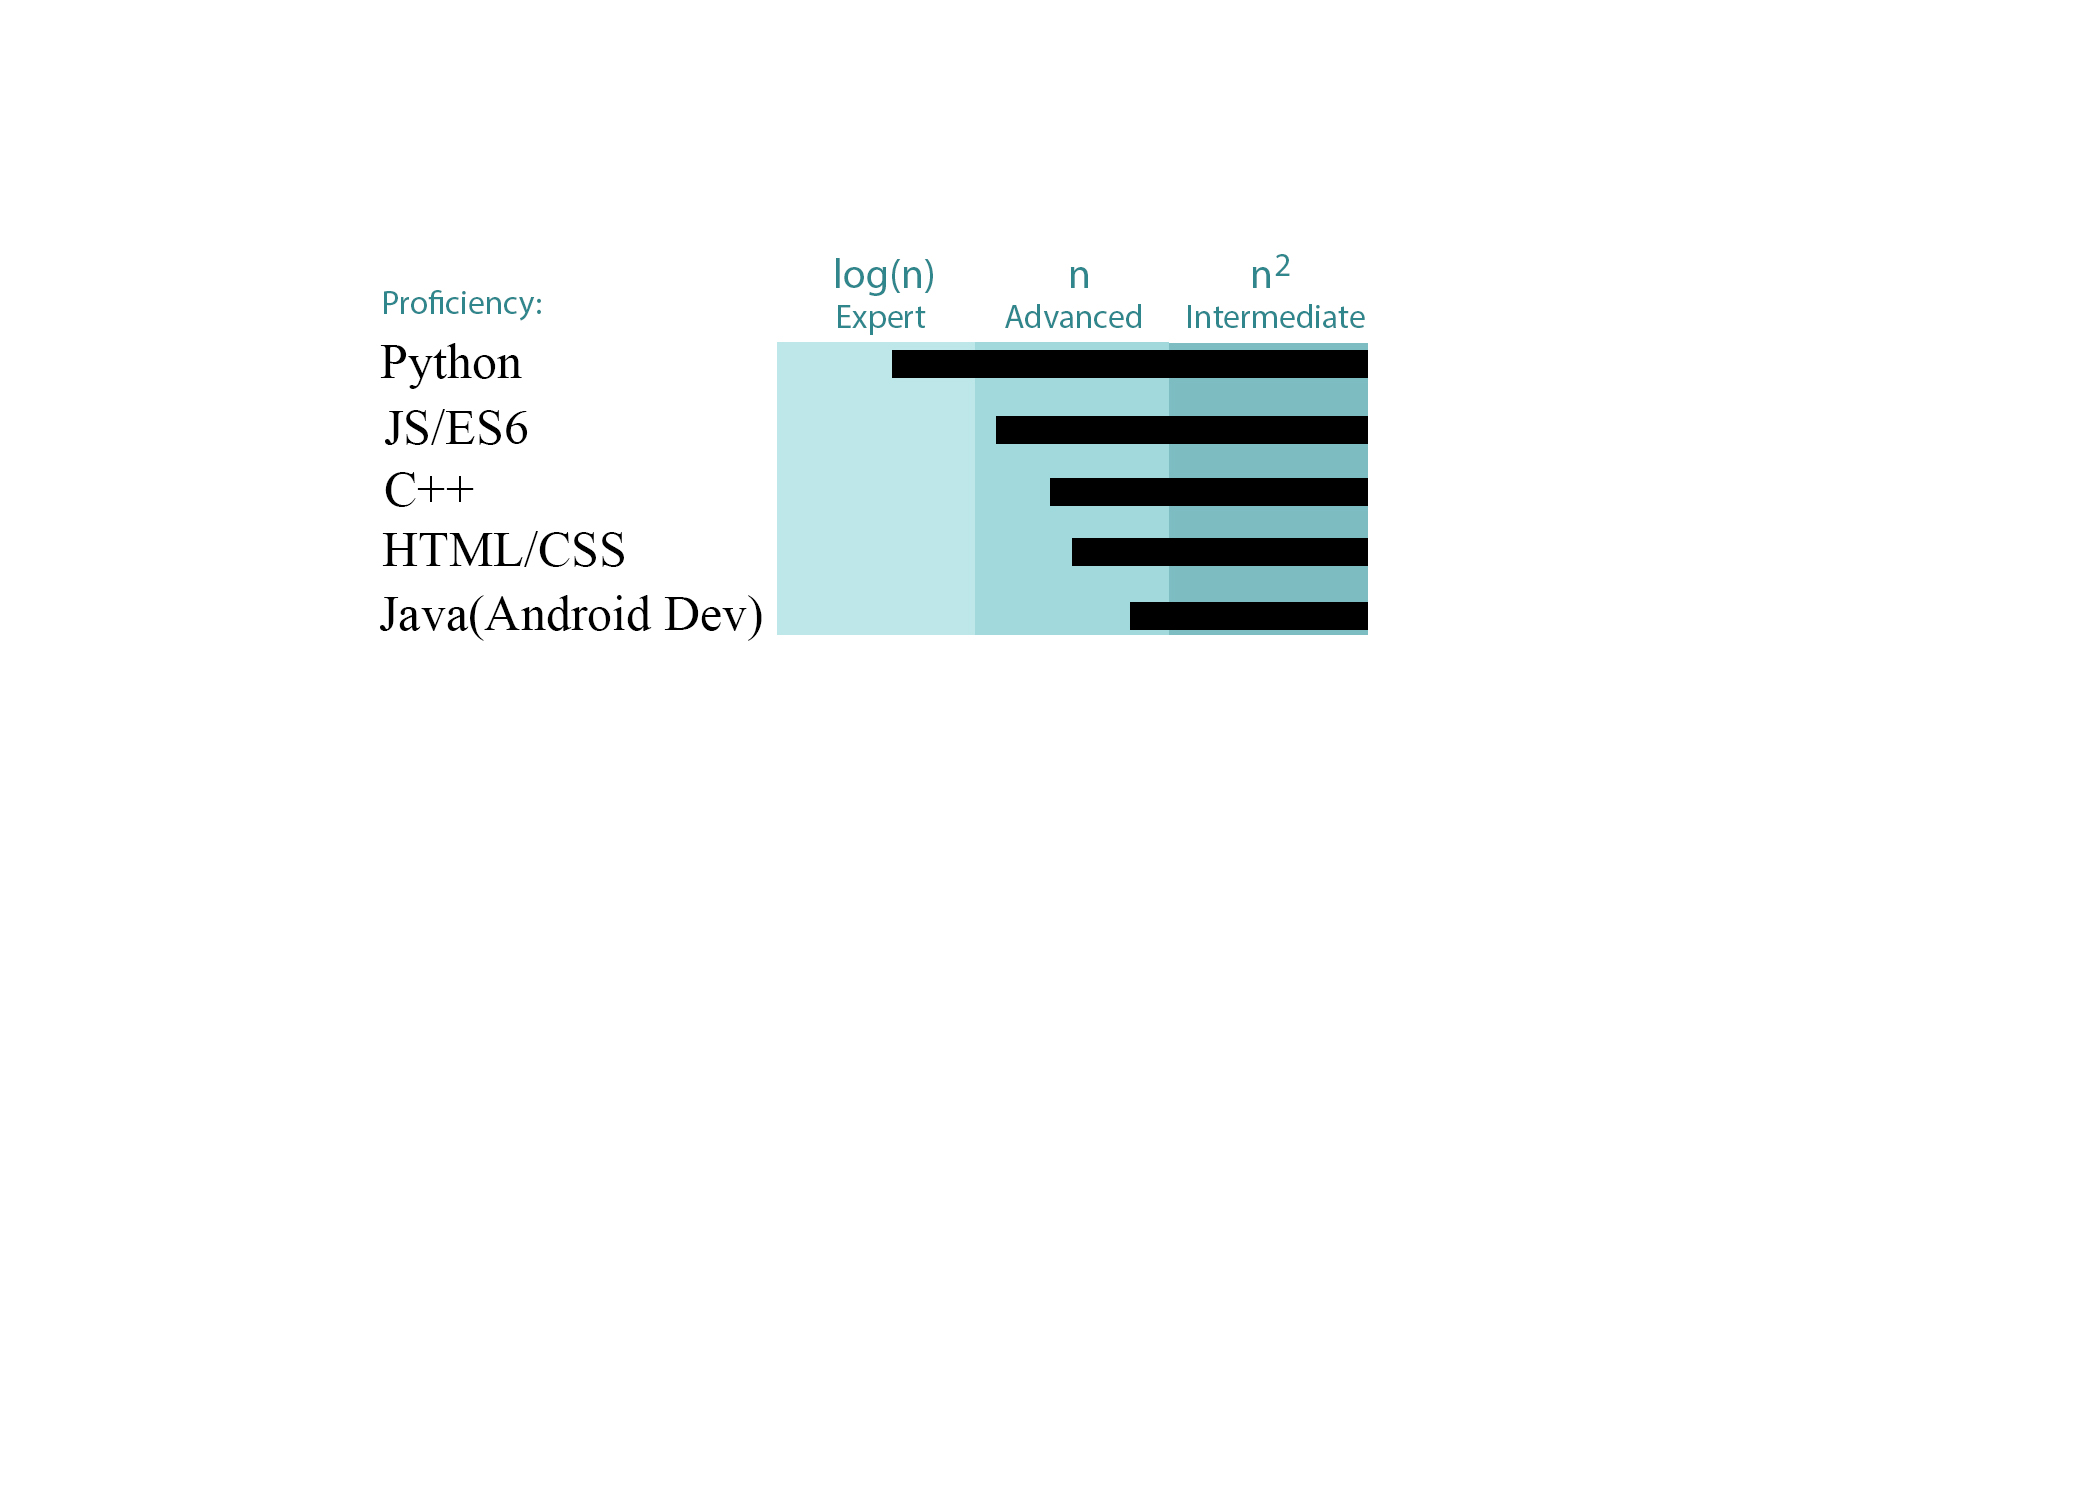
\includegraphics[trim={2.8cm 7cm 2cm 2cm},clip]{ResumePic}
\smallskip
\footnotesize
\color{gray}Git | Vim | Linux | Windows | MacOS | Android
\end{center}
\columnbreak
\center
\footnotesize
\color{black}\textsc{\textbf{ACM Club | CSU, Chico}}\\

\color{Cerulean}Algorithms Officer \hfill \color{gray}\textit{Current}\\
\begin{itemize}
\setlength{\itemsep}{0pt}
	\item Competed in Fall 2016 ACM Competition
	\item Research and present/teach algorithms at club meetings to be used during competition
\end{itemize}

\center
\color{black}\textsc{\textbf{Formula SAE Electric | CSU, Chico}}\\
\color{Cerulean}Member \hfill \color{gray}\textit{Current}

\begin{itemize}
\setlength{\itemsep}{0pt}
	\item Develop Formula SAE car to compete nationally
	\item Contribute to batteries and motor control team
\end{itemize}


\end{multicols}

\noindent\rule{19cm}{0.4pt}

\center
\color{black}
\color{black}
\begin{center}
\textbf{\textsc{-Internships-}}\\
\end{center}
\begin{footnotesize}
\flushleft
\color{Cerulean}\textbf{SocialHighRise}\hfill \color{TealBlue} \textbf{HTML/CSS/JS | jQuery | ASP.NET MVC | C\# | Razor | WordPress } \\ \color{Black}\textit{Software Development Intern} \hfill \textit{August 2016 - Current}
\color{black}
\begin{itemize}
    \setlength{\itemsep}{0pt}
	\item Develop in-house account manangement tool for organizing and monitoring social media profiles
	\item Manage all company tech support and IT needs including company website development
\end{itemize}
\color{Cerulean}\textbf{Lawrence Livermore National Laboratory} \color{Black} \hfill
\color{TealBlue} \textbf{PySide Qt | Python | HTML/CSS/JS | jQuery | React/Redux}\\
\color{Black} \textit{Computation Intern} \hfill\textit{Jan 2016 - August 2016} 
\color{Black}
\begin{itemize}
    \setlength{\itemsep}{0pt}
	\item Employed in a Co-op position, developing a Graphical User Interface for a large scale climate data visualization and analysis tool developed at the lab.
	\item Developed GUI in both PySide Qt and from scratch in HTML/CSS/JS, jQuery, React/Redux, and Flask

	\item Organized and presented demos of project to our team and communicated development timeline
	\item Collaborated with scientists using alpha, beta and previous versions of GUI to improve user experience and implement new functionality
\end{itemize}

\center
-Lab Hackathons-
\begin{multicols}{2}
\center
\color{Cerulean}ESGF Seach Client:\\ \color{black}
Recreated ESGF Search client for accessing\\
global climate data\\
Team Size: 2

\columnbreak

\color{Cerulean}JavaScript Distributed Multi Processing:\\ \color{black}
JavaScript library to distribute embarrassingly parallel problems over a large number of clients connected to a site\\
Team Size: 6


\end{multicols}
\medskip

\end{footnotesize}

\noindent\rule{19cm}{0.4pt}

\begin{center}
\textbf{\textsc{-Projects-}}\\
\end{center}
\begin{footnotesize}

\flushleft

\color{Cerulean}\textbf{Datasift Sentiment Visualization: \hfill \color{TealBlue} Node.js/Express | React | D3 | HTML/CSS/JS | jQuery} 
\color{Black}
\begin{itemize}
	\item Utilized Datasift Facebook Topic Data API trial to create visualization representing sentiment 
\end{itemize}
\smallskip
\flushleft
\color{Cerulean}\textbf{SnapStyle Fashion Social Media App: \hfill\color{TealBlue} Java/XML | Node.js/Express | MySql | Stormpath } 
\color{Black}
\begin{itemize}
	\item Fashion Social Media app developed to learn Android full stack
	\item Goal was to emphasize communication and suggestion for personal fashion
\end{itemize}
\smallskip

\end{footnotesize}

\center
Created with \LaTeX
\end{document}